\chapter{Gerador}
\label{cap:p1}


O \textit{generator} é um programa que é capaz de receber e interpretar pedidos do utilizador para desenho de figuras e gerar um ficheiro '.3d' com os pontos correspondentes à figura pedida. A lista de pontos está ordenada de forma a formarem triângulos que juntos desenham a figura desejada. 

Nesta primeira etapa, o objetivo implementar o suporte à criação de um plano, uma caixa, um cone e uma esfera. 


\section{Funcionamento}

Nesta primeira fase o \textit{generator} é capaz de criar diversas primitivas gráficas
diferentes, entre as quais: \textit{plane} (plano), \textit{box} (paralelepípedo), \textit{sphere} (esfera), \textit{cone}. Para cada uma das primitivas geométricas é possível gerar o ficheiro correspondente através dos comandos:

\begin{itemize}
	\item PLANE: generator plano/plane <comprimento largura> <ficheiro>, onde a largura e comprimento são opcionais 
	
	\item BOX: generator box/caixa <sizeX sixeY sizeZ divisões> <ficheiro>, onde existe a possibilidade de as divisões serem opcionais
	
	\item SPHERE: generator sphere/esfera <raio fatias camadas> <ficheiro>
	
	\item CONE: generator cone <raio altura fatias camadas> <ficheiro>
	
\end{itemize}


Para a criação das formas geométricas é preciso obedecer a algumas restrições
com a passagem de argumentos, o primeiro parâmetro a ser passado deverá
ser o nome da figura a desenhar, o último será o nome do ficheiro onde será
guardada a lista de pontos, sendo a extensão “.3d” adicionada automaticamente
pelo \textit{generator}. Sendo isto obedecido, o número de argumentos entre
o nome da figura e o nome do ficheiro varia consoante o tipo de figura a ser
criada, mas esses argumentos deverão ser numerais.

\newpage

\section{Algoritmo de Geração de Pontos}


\subsection{Gerar Planos}
\label{gp:plano}

\subsubsection{Plano em XZ (Y=constante)}

Um plano é formado por 2 triângulos. Com a informação de 4 pontos é possível desenhar esses triângulos. A figura \ref{p1:fig:p1_planoX} representa um plano em XZ. De notar que é possível considerar dois triângulos: o triângulo formado por [ABC] e o triângulo formado por [ACD]. 


\begin{figure}[<+htpb+>]
	\centering
	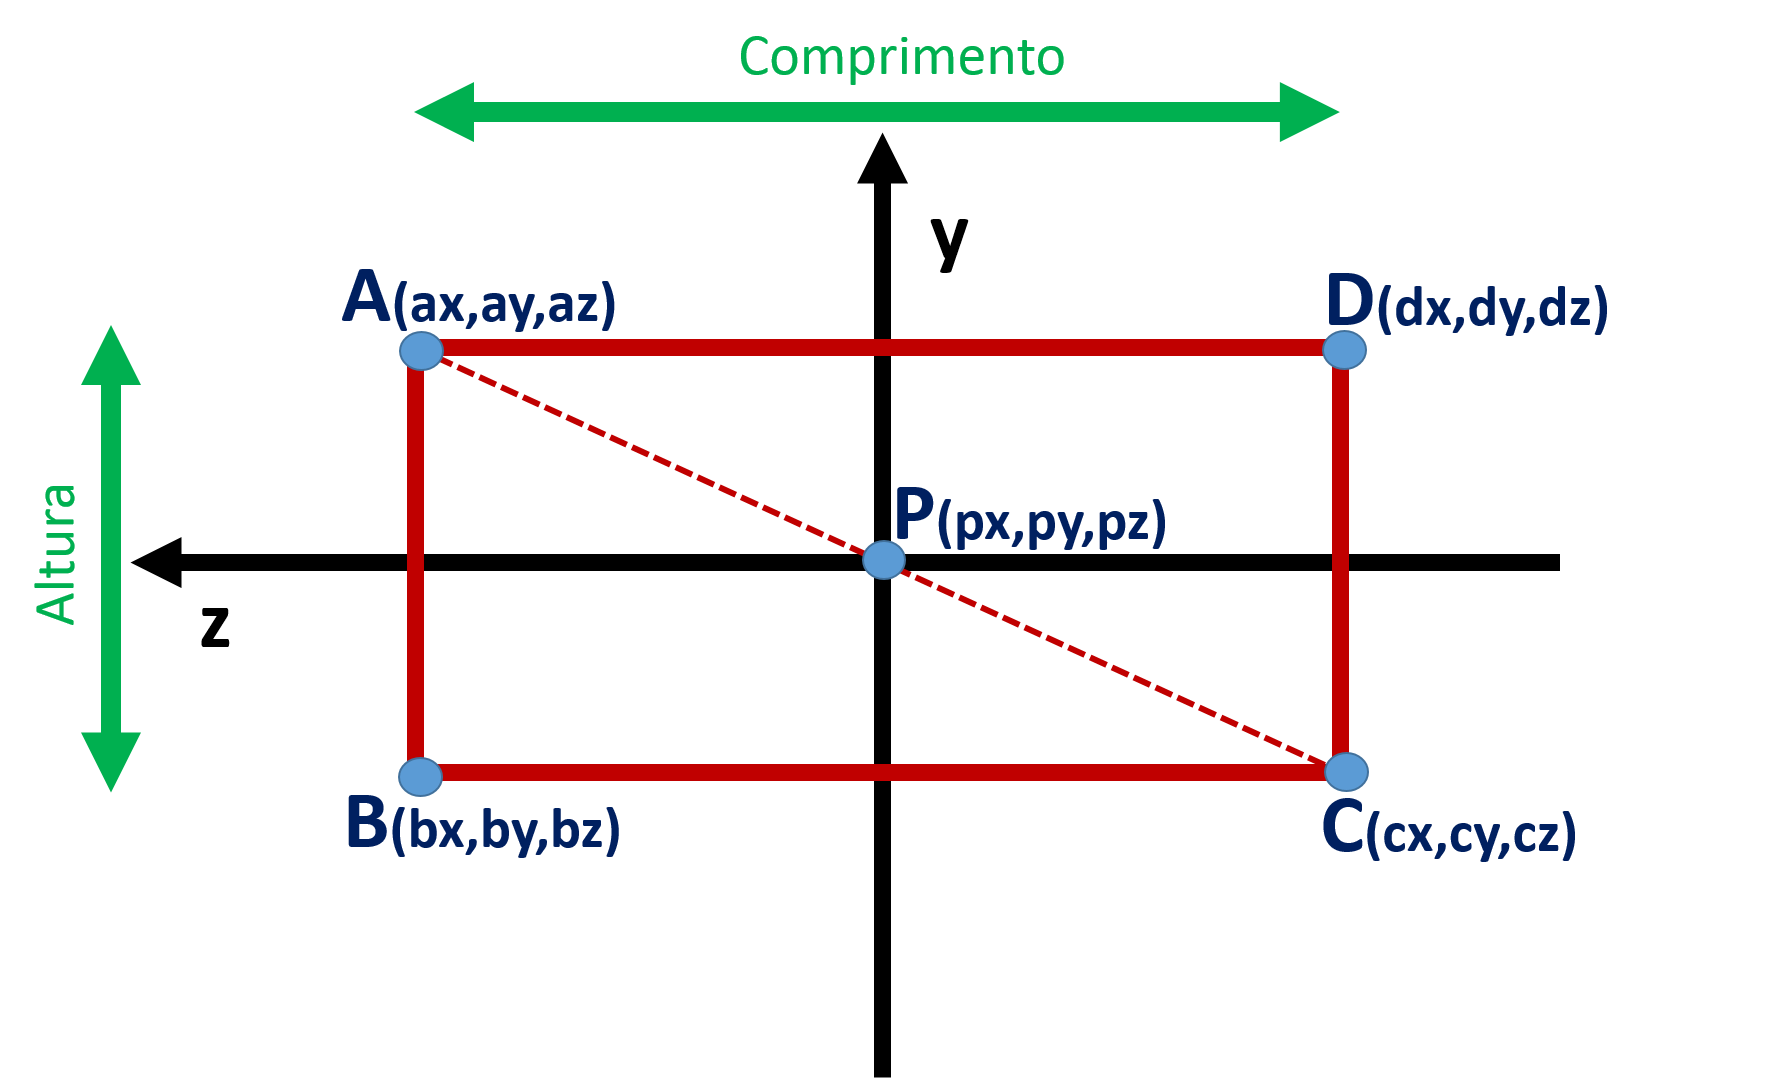
\includegraphics[scale=0.5]{imagens/p3_planoX.png}
	\caption{Plano em XZ centrado na origem}
	\label{p1:fig:p1_planoX}
\end{figure}


Estando o plano centrado na origem, e sabendo o comprimento e largura do plano, conclui-se que as coordenadas dos pontos da figura \ref{p1:fig:p1_planoX} são as seguintes:

\begin{Verbatim}
A(-largura/2, 0, comprimento/2)
B(largura/2, 0, comprimento/2)
C(largura/2, 0, -comprimento/2)
D(-largura/2, 0, -comprimento/2)
P(0, 0, 0)
\end{Verbatim}



A ordem pela qual se adiciona os pontos à figura determina para que lado ela fica virada. Se quisermos que o plano fique virado para o sentido positivo do eixo dos Y, deve-se colocar os pontos pela seguinte ordem: A-C-D (1º triângulo), seguido de A-B-C (2º triângulo). Se quisermos que o plano fique virado para o sentido negativo do eixo dos Y, deve-se colocar os pontos pela seguinte ordem: C-B-A (1º triângulo), seguido de D-C-A (2º triângulo).



De notar que esta função além do comprimento e largura, recebe ainda o centro do plano e a orientação do mesmo.

\begin{figure}[<+htpb+>]
	\centering
	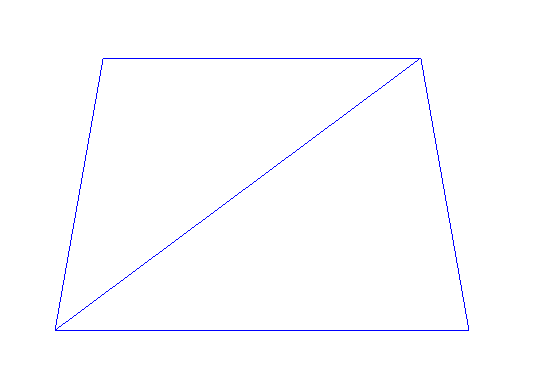
\includegraphics[scale=0.5]{imagens/p3_plano.png}
	\caption{Exemplo de plano em XZ gerado}
	\label{p1:fig:p3_plano_4_2}
\end{figure}


\newpage

\subsubsection{Plano em XY (Z=constante)}

Embora apenas fosse pedido que o gerador tivesse a capacidade de gerar um plano em XZ, considerou-se útil disponibilizar também uma primitiva para criar planos em XY.
Um plano é formado por 2 triângulos. Com a informação de 4 pontos é possível desenhar esses triângulos. A figura \ref{p1:fig:p3_planoY} representa um plano em XY. De notar que é possível considerar dois triângulos: o triângulo formado por [ABD] e o triângulo formado por [DBC]

\begin{figure}[<+htpb+>]
	\centering
	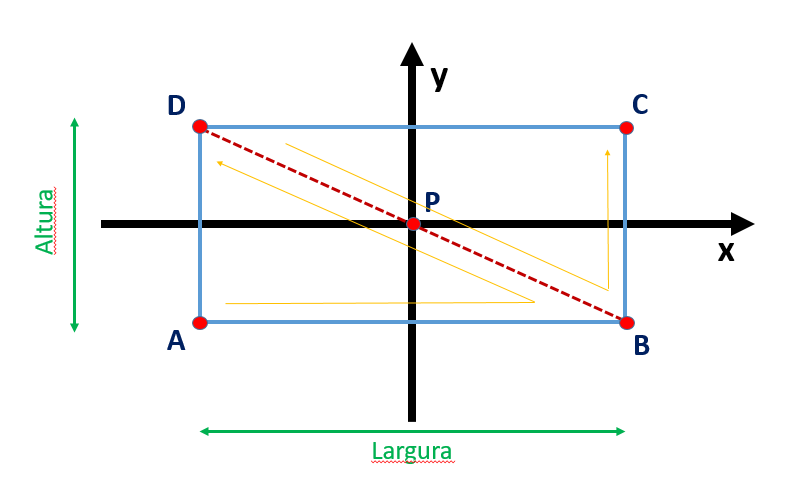
\includegraphics[scale=0.5]{imagens/p3_planoY.png}
	\caption{Plano em XY centrado na origem}
	\label{p1:fig:p3_planoY}
\end{figure}

Estando o plano centrado na origem, e sabendo o comprimento e largura do plano, conclui-se que as coordenadas dos pontos da figura \ref{p1:fig:p3_planoY} são as seguintes:

\begin{Verbatim}
A(-altura/2 , -largura/2, 0)
B(altura/2 , -lagura/2, 0)
C(altura/2 , largura/2, 0)
D(-altura/2 , lagura/2, 0)
P(0,0,0)
\end{Verbatim}



A ordem pela qual se adiciona os pontos à figura determina para que lado ela fica virada. Se quisermos que o plano fique virado para o sentido positivo do eixo dos Y, deve-se colocar os pontos pela seguinte ordem: A-B-D (1º triângulo), seguido de D-B-C (2º triângulo). Se quisermos que o plano fique virado para o sentido negativo do eixo dos Y, deve-se colocar os pontos pela seguinte ordem: C-B-D (1º triângulo), seguido de D-B-A (2º triângulo).


\subsubsection{Plano em YZ (X=constante)}

Embora apenas fosse pedido que o gerador tivesse a capacidade de gerar um plano em XZ, considerou-se útil disponibilizar também uma primitiva para criar planos em YZ.

Um plano é formado por 2 triângulos. Com a informação de 4 pontos é possível desenhar esses triângulos. A figura \ref{p1:fig:p3_planoZ} representa um plano em YZ. De notar que é possível considerar dois triângulos: o triângulo formado por [ ABC ] e o triângulo formado por [ DAC ].

\begin{figure}[<+htpb+>]
	\centering
	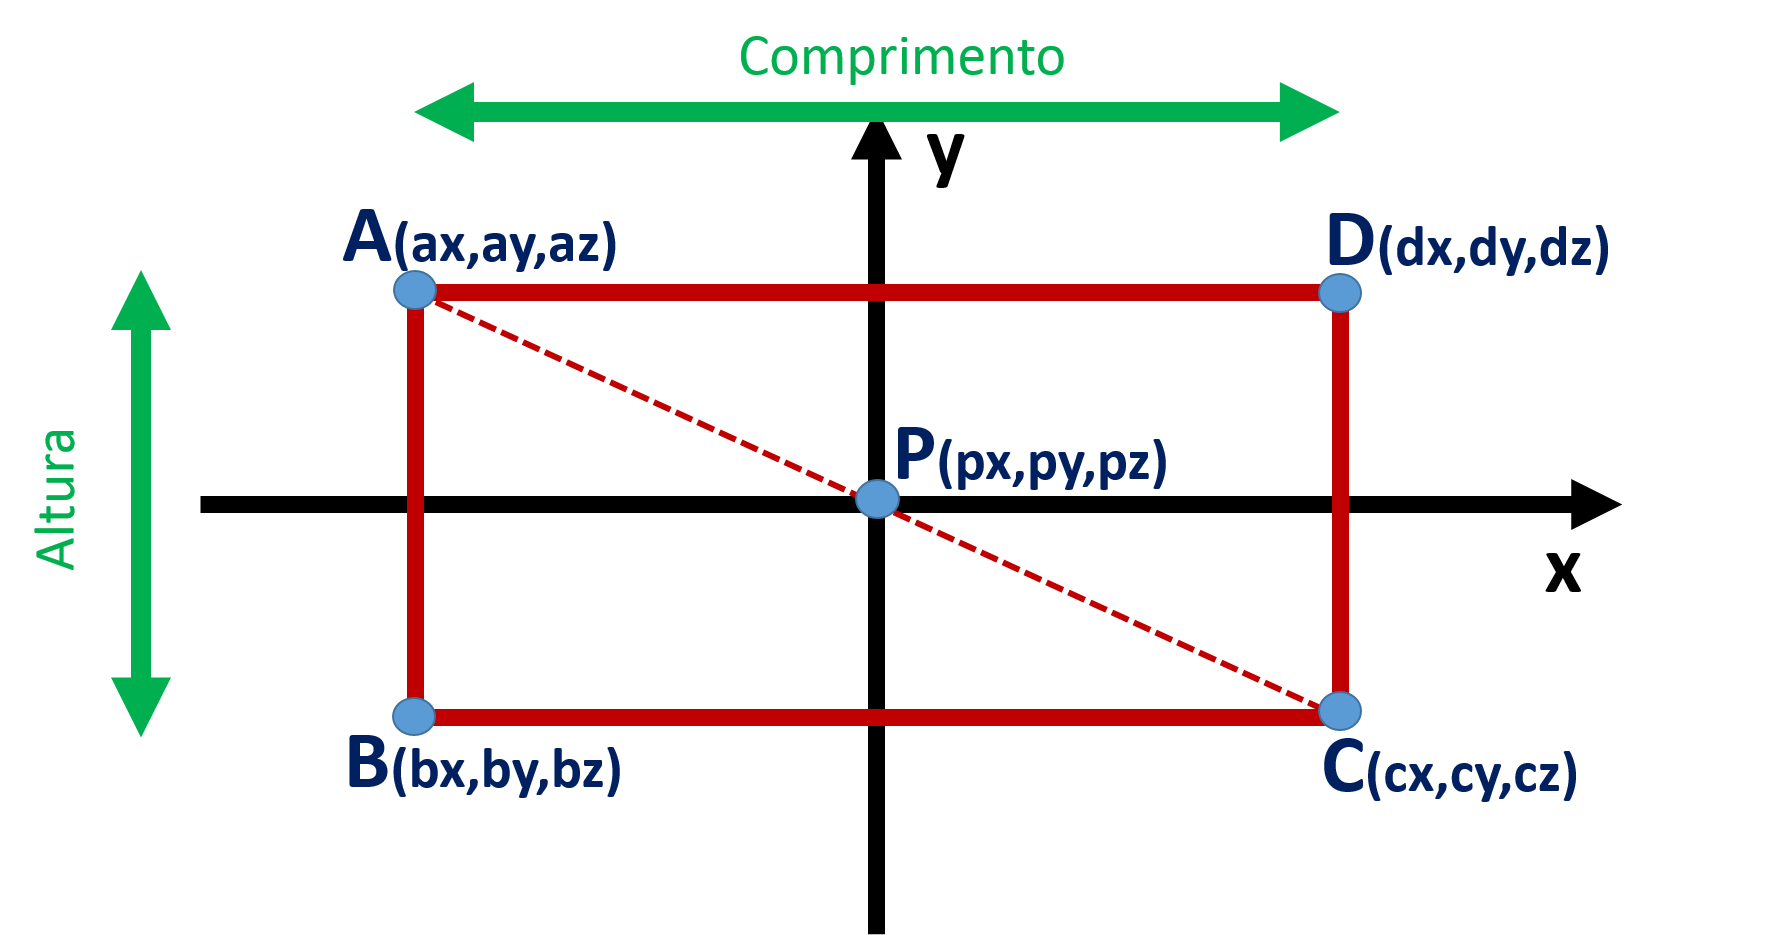
\includegraphics[scale=0.5]{imagens/p3_planoZ.png}
	\caption{Plano em XZ centrado na origem}
	\label{p1:fig:p3_planoZ}
\end{figure}

Estando o plano centrado na origem, e sabendo o comprimento e largura do plano, conclui-se que as coordenadas dos pontos da figura \ref{p1:fig:p3_planoZ} são as seguintes:

\begin{Verbatim}
A(0, -comprimento/2, altura/2)
B(0, -comprimento/2, -altura/2)
C(0, comprimento/2, -altura/2)
D(0, comprimento/2, altura/2)
P(0,0,0)
\end{Verbatim}


A ordem pela qual se adiciona os pontos à figura determina para que lado ela fica virada. Se quisermos que o plano fique virado para o sentido positivo do eixo dos Y, deve-se colocar os pontos pela seguinte ordem: A-B-C (1º triângulo), seguido de D-A-C (2º triângulo). Se quisermos que o plano fique virado para o sentido negativo do eixo dos Y, deve-se colocar os pontos pela seguinte ordem: C-A-D (1º triângulo), seguido de C-B-A (2º triângulo).
\\

A função responsável por implementar estes algoritmos é a função \textit{drawPlane\_Points()}, que funciona do seguinte modo: quando queremos desenhar em ordem a um plano, esse plano tem valor zero, cujo pseudo-código se apresenta de seguida:

\begin{Verbatim}
drawPlane_Points(float sizeX, float sizeY, float sizeZ, 
float centerX, float centerY, float centerZ, int divisions,
bool rev, Ponto3D points){

Calcula coordendas dos pontos A,B,C e D

if (rev == 0) {
Desenha os pontos contra-relógio

}
else {
Desenha no sentido do relogio

}

return número de pontos calculados;
}
\end{Verbatim}



\subsection{Gerar Caixa}


Na secção \ref{gp:plano} foram apresentadas as primitivas que permitiam fazer planos. Nomeadamente viu-se que essas primitivas permitiam gerar planos em XY, YZ e XZ dado um centro e uma orientação.

Uma caixa é apenas um conjunto de planos. Assim, para gerar a caixa o que se fez foi gerar os seus planos usando as primitivas da secção \ref{gp:plano}. No entanto, para usar tais primitivas é necessário indicar um centro do plano e uma orientação para o mesmo. É por isso necessário calcular esses parâmetros antes de usar as primitivas dos planos.

Considere-se a caixa com as faces visíveis identificadas pelas letras A, B e C, conforme mostra a figura \ref{p1:fig:p3_Caixa}

\begin{figure}[<+htpb+>]
	\centering
	\includegraphics[scale=0.5]{imagens/p3_Caixa.png}
	\caption{Esquema representativo da caixa}
	\label{p1:fig:p3_Caixa}
\end{figure}

Considere-se ainda que a face oposta a A é designada por A', a face oposta a B por B' e a face oposta a C por C'.
Interessa agora saber as coordenadas dos centros de cada uma destas faces. Considerando a caixa centrada na origem, temos o seguinte:

\begin{Verbatim}
Centro A  = (0,altura/2,0)          Orientação = 0
Centro A' = (0,-altura/2,0)         Orientação = 1
Centro B  = (largura/2,0,0)         Orientação = 0
Centro B' = (-largura/2,0,0)        Orientação = 1
Centro C  = (0,0,comprimento/2)     Orientação = 0
Centro C' = (0,0,-comprimento/2)    Orientação = 1
\end{Verbatim}

\newpage


A função responsável por gerar os pontos de uma caixa é a função \textit{drawBox\_Points()} cujo pseudo-código se apresenta a seguir:

\begin{Verbatim}


drawBox_Points(float sizeX, float sizeY, float sizeZ, 
float centerX, float centerY, float centerZ, int divisions, 
Ponto3D points){

Calcula coordendas centro A
Cria plano com centro em A e orientacao = 0

Calcula coordendas centro A'
Cria plano com centro em A' e orientacao = 1

Calcula coordendas centro B
Cria plano com centro em B e orientacao = 0

Calcula coordendas centro B'
Cria plano com centro em B' e orientacao = 1

Calcula coordendas centro C
Cria plano com centro em C e orientacao = 0

Calcula coordendas centro C'
Cria plano com centro em C' e orientacao = 1

return número de ponto que calculou para fazer a caixa;
}

\end{Verbatim}

\begin{figure}[<+htpb+>]
	\centering
	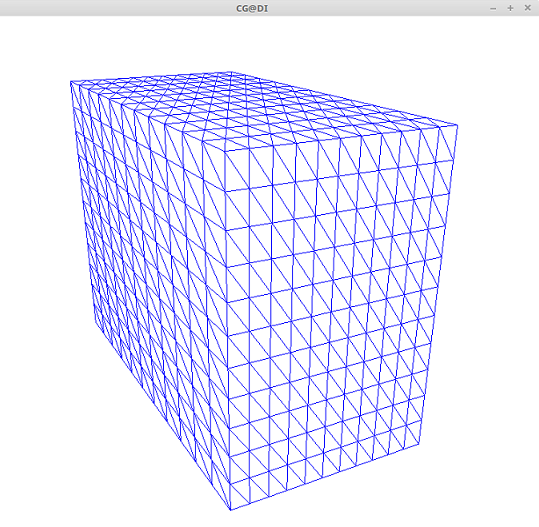
\includegraphics[scale=0.5]{imagens/p3_caixa_10.png}
	\caption{Exemplo de caixa gerada}
	\label{p1:fig:p3_caixa_6_3_4}
\end{figure}



\subsection{Gerar Cone}

Para gerar os pontos do cone, primeiro é necessário desenhar os pontos da camada do topo do cone, estes que serão a primeira camada constituida apenas por triângulos. 


De seguida é necessário gerar os pontos para a superfície ``curva'' do cone. Para essa superfício, abordagem seguida foi a de fazer o cone camada a camada. As fatias partem cada camada numa espécie ``rectângulos'' como o que se mostra na figura \ref{p1:fig:p3_seccaoCone_edit}.


\begin{figure}[<+htpb+>]
	\centering
	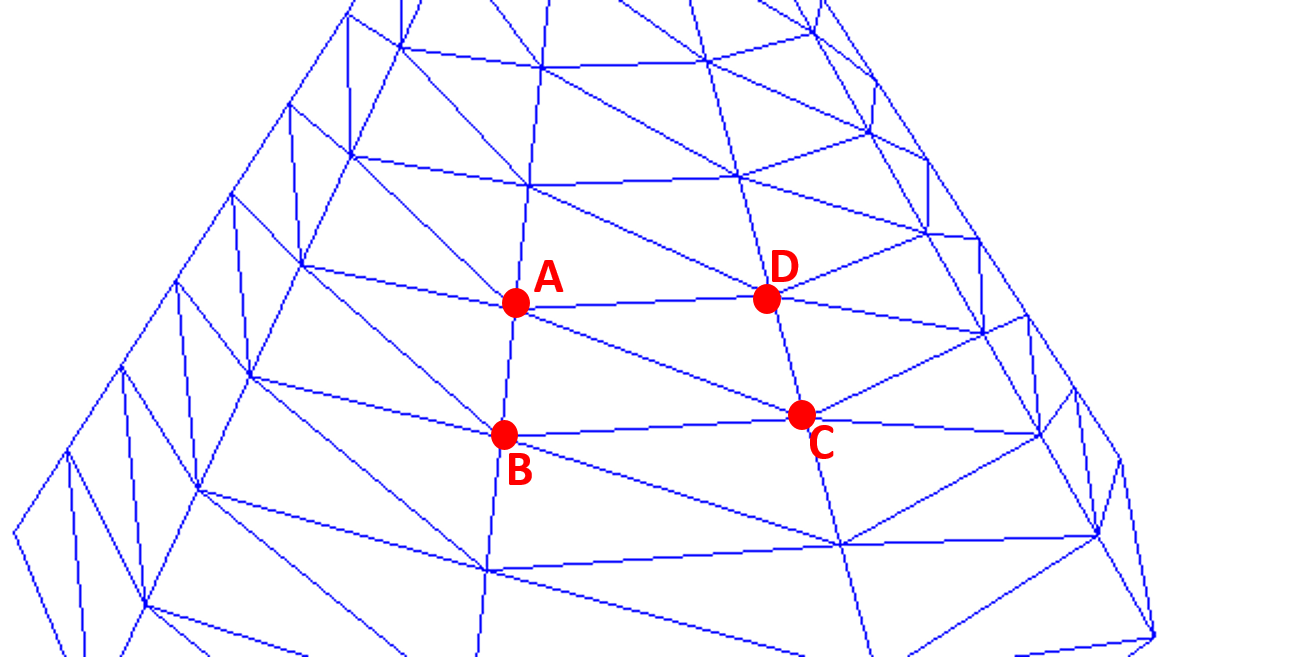
\includegraphics[scale=0.5]{imagens/p3_seccaoCone_edit.png}
	\caption{Esquema representativo de uma fatia de uma camada do cone (Pontos A,B,C e D)}
	\label{p1:fig:p3_seccaoCone_edit}
\end{figure}

Ou seja, é possível construir uma fatia de uma dada camada com os pontos A,B,C e D. É no entanto necessário saber as coordenadas destes pontos. Para tal, foram usadas coordenadas polares. Podemos ver os pontos A e D como pertencentes a um mesmo círculo, com centro no centro do cone. Da mesma forma, também os pontos B e C se encontram num mesmo círculo, com raio maior do que o círculo onde estão os pontos A e D. O raio dos dois círculos em que estes dois conjuntos de pontos se encontram difere, no entanto o raio do círculo depende da camada que se está a considerar. 


Por exemplo, se virmos a base do cone como um círculo de raio $Raio$, à medida que o valor de $Altura$ aumenta, ou seja, à medida que subimos no cone, o $Raio$ das novas circunferências vai sendo cada vez menor.
Quando $Altura$ for igual ao valor de $d$ o raio da nova circunferência é
0, ou seja, é apenas o ponto do topo do cone.  A figura \ref{p1:fig:p3_conePerfil} pretende ilustrar tal situação. 

\begin{figure}[<+htpb+>]
	\centering
	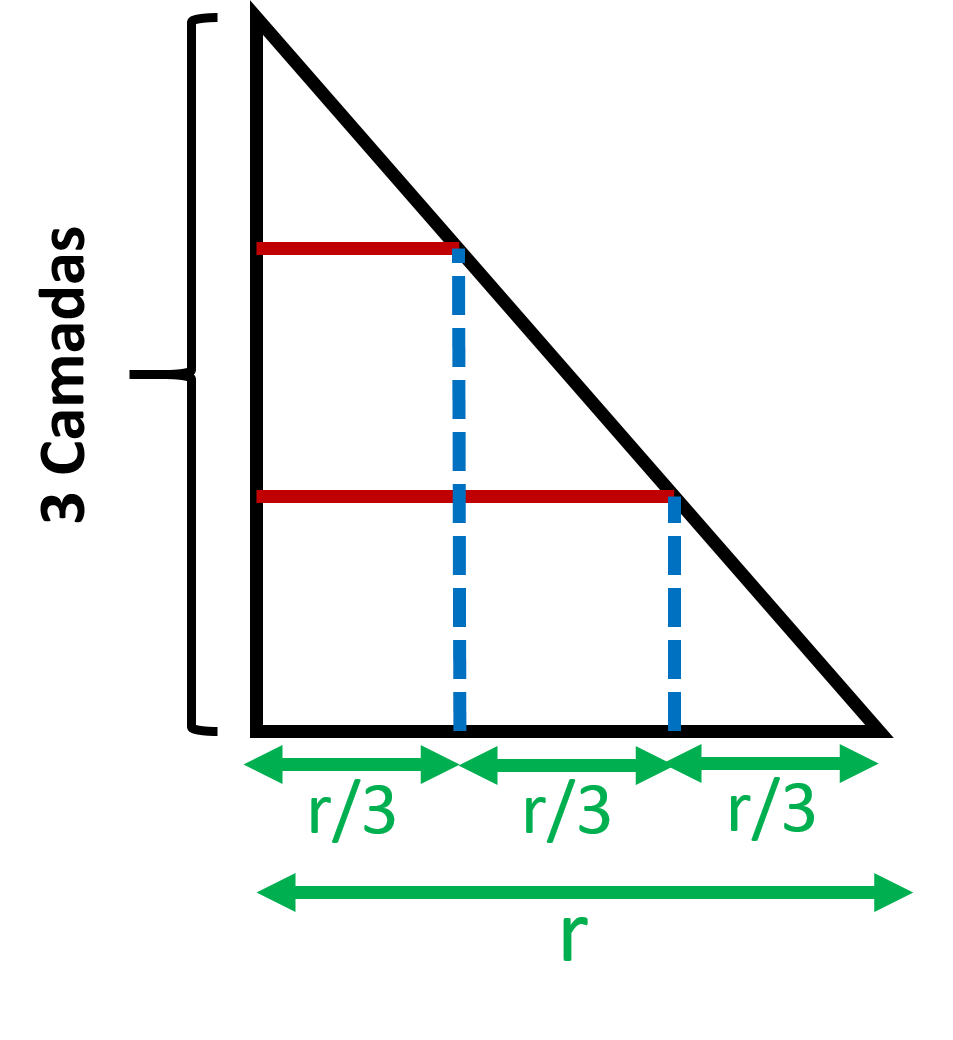
\includegraphics[scale=0.5]{imagens/p3_conePerfil.png}
	\caption{Cálculo da altura de cada camada do cone $d = (altura/camadas)$}
	\label{p1:fig:p3_conePerfil}
\end{figure}

A função \textit{drawCone\_Points} permite desenhar um cone e o seu pseudo-código é mostrado de seguida: 

\begin{Verbatim}

drawCone_Points(float radius, float height, float centerX, 
float centerY, float centerZ, int slices, int stacks, 
Ponto3D points){

sinAlpha = radius / height;//calcula os raios das diferentes stacks;

divBeta = (360.0f / (float) slices) * M_PI / 180.0f;//tamanho do 
ângulo para cada slice

d = height / (float) stacks; // altura de cada stack do cone

for(i = 1;i < slices;i++)
	Calcula ângulos no plano paralelo a XZ (chao);
	
for(i = 0;i < slices; i++)	{
	Desenha os triângulos do topo do cone 
}


for(i = 2;i <= stacks;i++){
	for(j = 0;j < slices;j++){
		Desenha os quadradros até à base do cone
	}
}
	
for(i = 0; i < slices; i++){
	Desenha o circulo (base do cone)
	}
}

\end{Verbatim}


\begin{figure}[<+htpb+>]
	\centering
	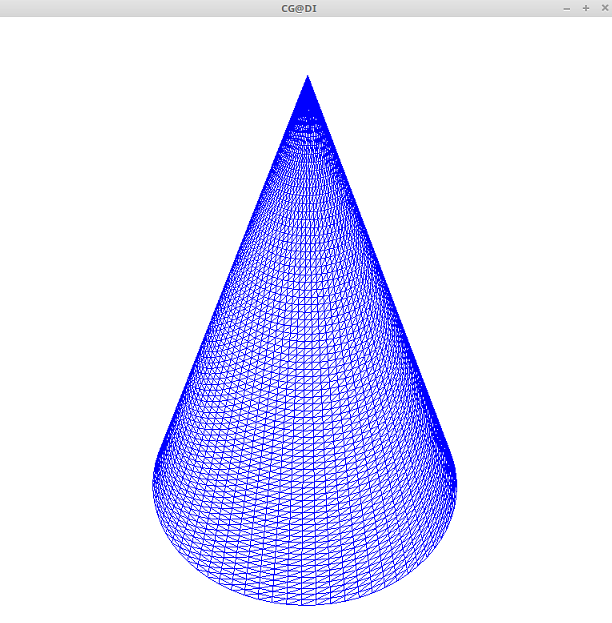
\includegraphics[scale=0.5]{imagens/print_cone_raio1-5_altura4_slices75_stacks75}
	\caption{Exemplo de cone gerado com raio 1.5,altura 4, 75 fatias, 75 camadas}
	\label{p1:fig:p3_cone_2_3_10_10}
\end{figure}


\newpage
\subsection{Gerar Esfera}

À semelhança do cone também para a esfera é possível gerar uma fatia de uma determinada camada usando 4 pontos conforme mostrado na figura \ref{p1:fig:p3_esferaSeccao_edit}.

\begin{figure}[<+htpb+>]
	\centering
	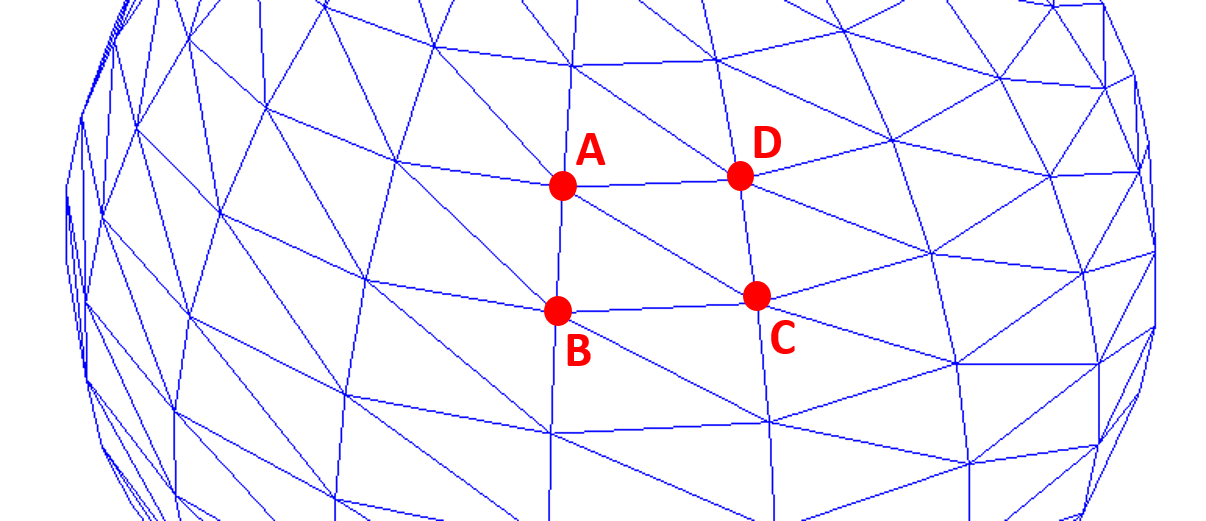
\includegraphics[scale=0.5]{imagens/p3_esferaSeccao_edit.png}
	\caption{Esquema representativo de uma fatia de uma camada da esfera (Pontos A,B,C e D)}
	\label{p1:fig:p3_esferaSeccao_edit}
\end{figure}

Também para a esfera a abordagem seguida foi a de construir camada a camada, começando pelos topos na direção do eixo dos YY e o centro paralelo ao plano XZ. 
O centro da esfera é o ponto de coordenadas (0, 0, 0) e vão ser necessários dois ângulos diferentes para conseguir desenhar os triângulos que ligam as diferentes circunferências.

Utiliza-se um arco no plano XY divido em partes iguais, dependendo do
número de stacks. O ângulo dentro desse arco será $\beta$ e para cada um dos
valores de $\alpha$ é possível obter o valor de y para a nova circunferência assim
como o raio da mesma.
Cada uma das circunferências vai ser dividida em partes iguais, dependendo
do número de slices. Para calcular os diferentes pontos dentro da
circunferˆencia utiliza-se um ângulo  $\alpha$ e, para cada um dos pontos criam-se
dois triângulos ligados à circunferência imediatamente abaixo, um à direita
do ponto atual e outro à esquerda. 


Tal como no cone a criação dos arrays com os ângulos todos, as fatias  e as camadas sendo que os iniciais sao predefinidos
, os angulos alpha (do Norte ao sul) começam em 90 e vao até -90, i.e., $\pi /2 $e vão até $-\pi /2 $
 

Assim temos o seguinte pseudo-código:

\begin{Verbatim}

drawSphere(float radius, float centerX, float centerY, float centerZ, int stacks, int slices, Ponto3D points){

// calculo do angulo de cada slice e stack, passado para radianos
divBeta = (360.0f / (float) slices) * M_PI / 180.0f;
divAlpha = M_PI / (float) stacks;  


for(i = 0;i < slices; i++){
Desenha os triângulos da parte superior da esfera;
Desenha os triângulos da parte inferiro da esfera;
}

for(i = 2;i <= stacks;i++){
	for(j = 0;j < slices;j++){
Desenha quadrados para completar o resto da esfera
	}
}

}

\end{Verbatim}

\begin{figure}[<+htpb+>]
	\centering
	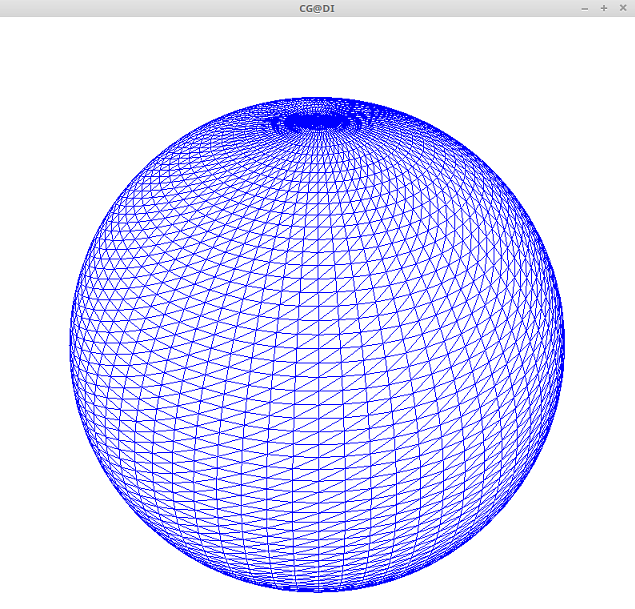
\includegraphics[scale=0.5]{imagens/p3_esfera_2_75_75.png}
	\caption{Exemplo de esfera gerada com raio 2, 75 camadas e 75 fatias}
	\label{p1:fig:p3_esfera_2_20_20}
\end{figure}




